\documentclass[11pt]{article}
\usepackage{graphicx}
\usepackage{hyperref}
\usepackage{natbib}
\usepackage{amsmath}
\usepackage{enumitem}

\setlength{\textwidth}{6.5in}
\setlength{\headheight}{0in}
\setlength{\textheight}{8.0in}
\setlength{\hoffset}{0in}
\setlength{\voffset}{0in}
\setlength{\oddsidemargin}{0in}
\setlength{\evensidemargin}{0in}

\title{PS5}
  
\author{Shihong Pan\\ \url{https://github.com/PSH-hub24/phys-ga2000}}


\begin{document}

\maketitle

\section{Q1}
Fig \ref{fig:Q1CD} plots the numerical and analytic result of the derivative of $f(x)$ using a central difference. Fig \ref{fig:Q1Jax} plots the numerical and analytic result of the derivative of $f(x)$ using the jax package which does work as advertised. 

\section{Q2}
\begin{enumerate}[label=(\alph*)]
    \item Fig \ref{fig:Q2a} plots the curves of the integrand with $a=2,3,4$.
    \item Take the first and second derivative of the integrand:
    \begin{align}
        D_1 &= \frac{d}{dx}(x^{a-1}e^{-x})=(a-1)x^{a-2}e^{-x}-x^{a-1}e^{-x}\\
        D_2 &= \frac{d^2}{dx}(x^{a-1}e^{-x})=(a-1)(a-2)x^{a-3}e^{-x}-(a-1)x^{a-2}e^{-x}-D_1
    \end{align}
    It is clear that substituting $x=a-1$ gives $D_1=0$ and $D_2<0$, i.e, the maximum falls at $x=a-1$.
    \item If $x=c$ then $z=1/2$. Since the peak is at $x=a-1$, pick $c=a-1$.
    \item The integrand becomes
    \begin{align}
        e^{(a-1)\ln(x)}e^{-x}=e^{(a-1)\ln(x)-x}
    \end{align}
    The new expression is better because we are now only evaluating one exponential, and the value of $(a-1)\ln(x)-x$ suffers less from large $x$ since we are subtracting two large terms at large $x$.
    \item Fig \ref{fig:Q2GammaValues} prints the values of $\Gamma(a)$ for $a=3/2,3,6,10$, the answers for both part (e) and (f).
    \item See above.
\end{enumerate}

\section{Q3}
\begin{enumerate}[label=(\alph*)]
    \item Fig \ref{fig:Q3a} plots the signal data.
    \item Fig \ref{fig:Q3b} plots the best third-order polynomial fit in time to the signal, using the SVD technique.
    \item Fig \ref{fig:Q3c} plots the residuals of the data wrt the model. This is not a good explanation of the data, because the RMSE value I calculated is around 2.526 which is a bit far away from the given standard deviation 2.0. Please see my codes for all the RMSE calculations.
    \item Fig \ref{fig:Q3dFit} plots the model and data with the order of polynomial equals to 30. The conditional number of the corresponding $A$ is around 2.74e12 which I think is still a reasonable value (and it does produce a reasonable curve). I also plot the residuals in Fig \ref{fig:Q3dResidual}, and the corresponding RMSE value is $2.006$ which is pretty close to the standard deviation of the signal data.
    \item Fig \ref{fig:Q3eFit} plots the Lomb-Scarge model and the signal data, and Fig \ref{fig:Q3eResidual} plots the residuals. The RMSE value is 2.014 which is also close to the standard deviation of the data. The model looks like a reasonbale fit since the typical periodicity of the data is clearly shown by the orange curve.
\end{enumerate}

\begin{figure}[b!]
\centering
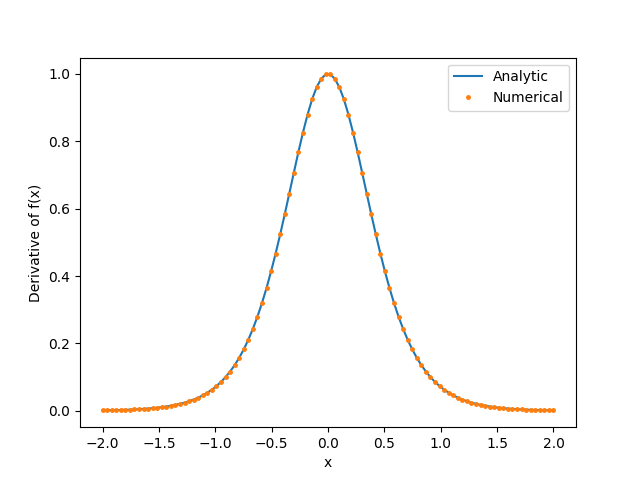
\includegraphics[width=0.6\textwidth]{Computational Physics/ps5Figures/q1CentralDiff.png}
\caption{Q1: Derivative of f(x) using central difference.}
  \label{fig:Q1CD}
\end{figure}

\begin{figure}[b!]
\centering
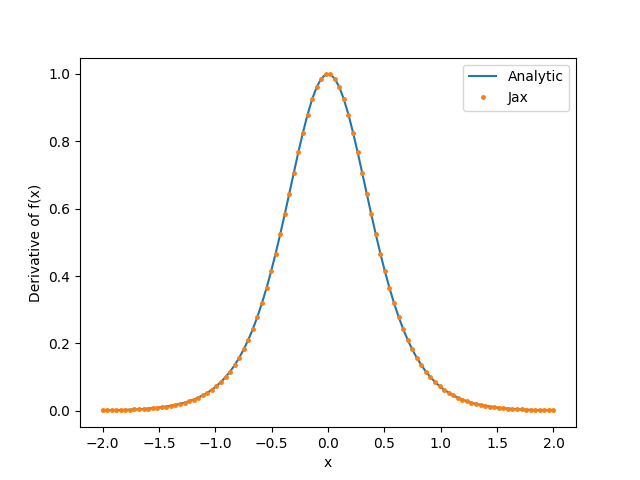
\includegraphics[width=0.6\textwidth]{Computational Physics/ps5Figures/q1Jax.png}
\caption{Q1: Derivative of f(x) using Jax.}
  \label{fig:Q1Jax}
\end{figure}

\begin{figure}[b!]
\centering
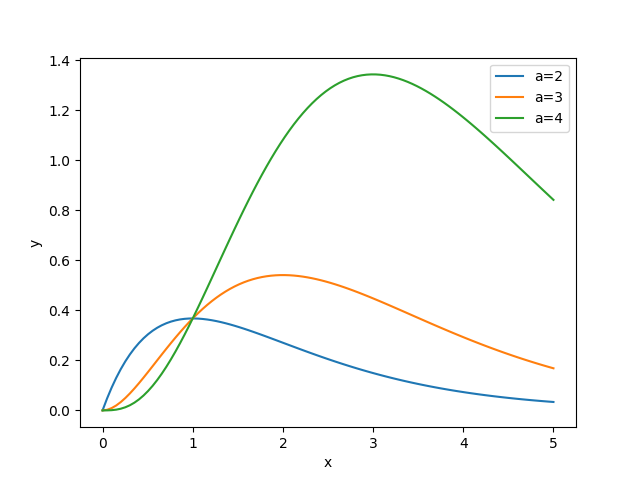
\includegraphics[width=0.6\textwidth]{Computational Physics/ps5Figures/q2a.png}
\caption{Q2(a): Three separate curves for $a=2,3,4$.}
  \label{fig:Q2a}
\end{figure}

\begin{figure}[b!]
\centering
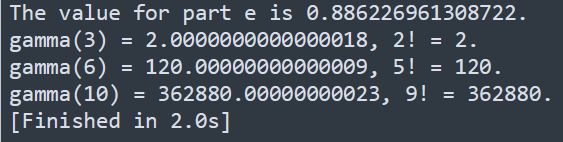
\includegraphics[width=0.6\textwidth]{Computational Physics/ps5Figures/q2GammaValues.PNG}
\caption{Q2(e),(f): The values of $\Gamma(a)$ for $a=3/2, 3, 6, 10$.}
  \label{fig:Q2GammaValues}
\end{figure}

\begin{figure}[b!]
\centering
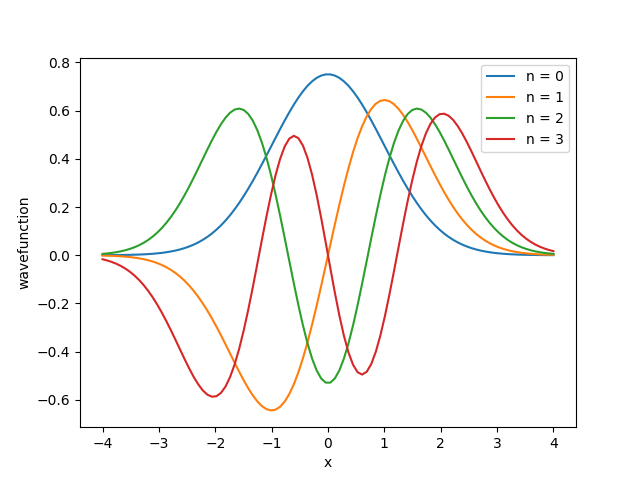
\includegraphics[width=0.6\textwidth]{Computational Physics/ps5Figures/q3a.png}
\caption{Q3(a): The scatter plot of raw signal data.}
  \label{fig:Q3a}
\end{figure}

\begin{figure}[b!]
\centering
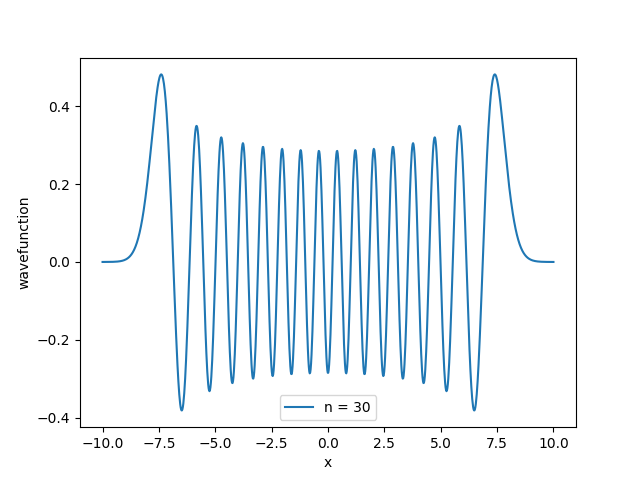
\includegraphics[width=0.6\textwidth]{Computational Physics/ps5Figures/q3b.PNG}
\caption{Q3(b): The best third-order polynomial fit in time to the signal, using the SVD technique.}
  \label{fig:Q3b}
\end{figure}

\begin{figure}[b!]
\centering
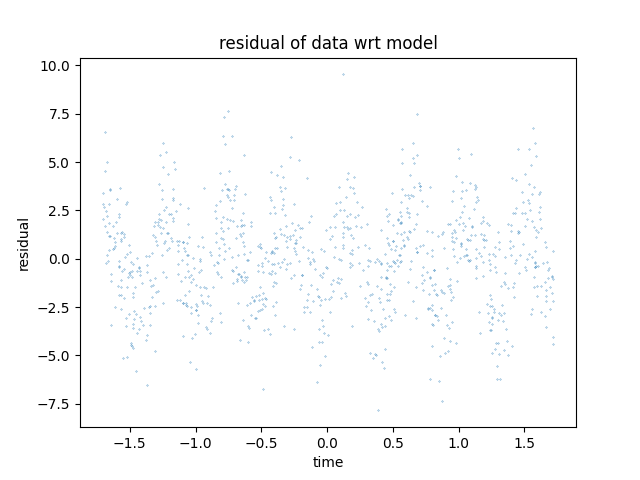
\includegraphics[width=0.6\textwidth]{Computational Physics/ps5Figures/q3c.PNG}
\caption{Q3(c): The residuals of the data wrt the model in part (b).}
  \label{fig:Q3c}
\end{figure}

\begin{figure}[b!]
\centering
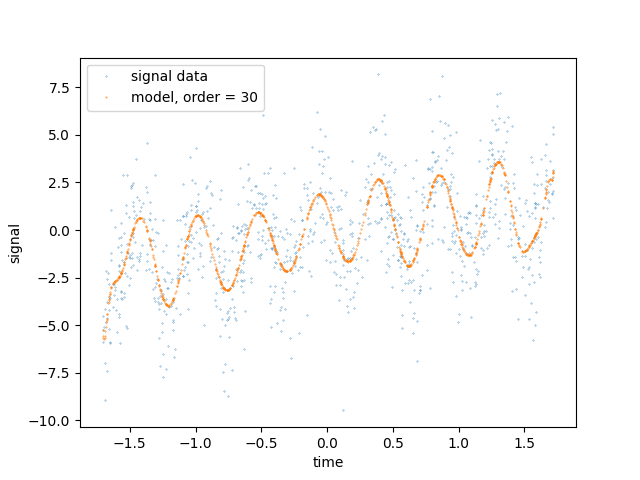
\includegraphics[width=0.6\textwidth]{Computational Physics/ps5Figures/q3dFit.png}
\caption{Q3(d): The signal data and the model with the order of polynomial = 30.}
  \label{fig:Q3dFit}
\end{figure}

\begin{figure}[b!]
\centering
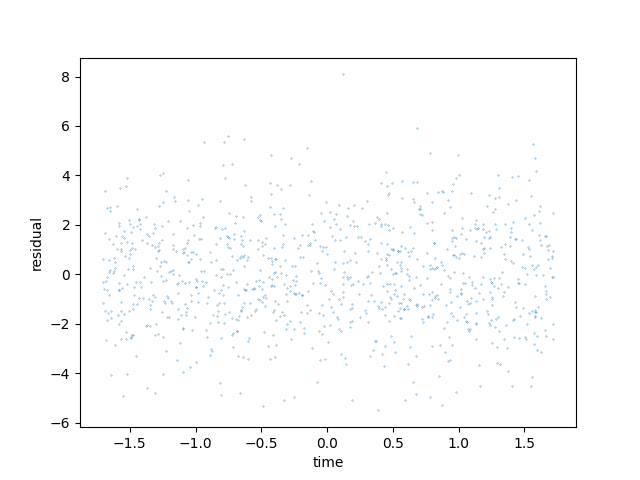
\includegraphics[width=0.6\textwidth]{Computational Physics/ps5Figures/q3dResidual.png}
\caption{Q3(d): The residuals of the data wrt the model with the order of polynomial = 30.}
  \label{fig:Q3dResidual}
\end{figure}

\begin{figure}[b!]
\centering
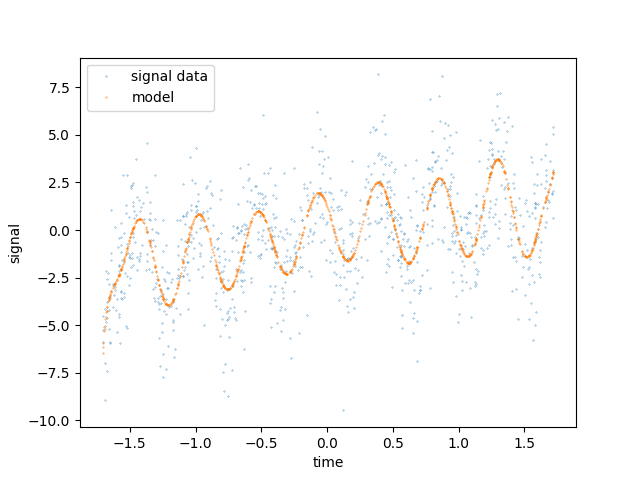
\includegraphics[width=0.6\textwidth]{Computational Physics/ps5Figures/q3eFit.png}
\caption{Q3(e): Use the Lomb-Scargle model to fit the data.}
  \label{fig:Q3eFit}
\end{figure}

\begin{figure}[b!]
\centering
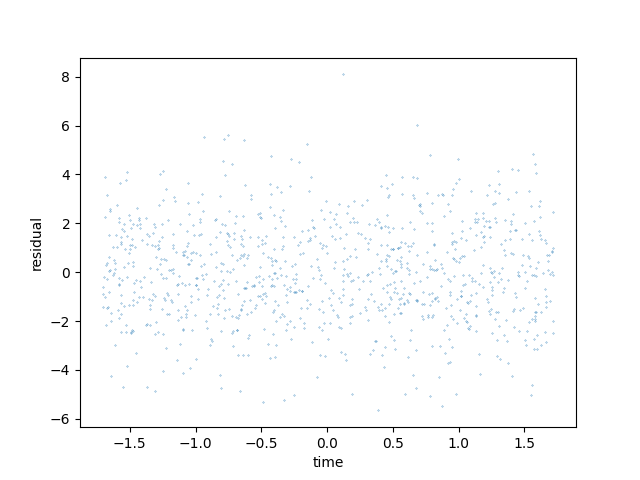
\includegraphics[width=0.6\textwidth]{Computational Physics/ps5Figures/q3eResidual.png}
\caption{Q3(e): The residuals of the data wrt the Lomb-Scargle model.}
  \label{fig:Q3eResidual}
\end{figure}

\bibliographystyle{apj}
\bibliography{example}

\end{document}

 
 
